\section{Entwurfsmuster (8P)}
\task{2 unterschiedliche Entwurfsmuster aus der Vorlesung (oder nach Absprache auch andere) jeweils benennen, sinnvoll einsetzen, begründen und UML-Diagramm}
\subsection{Entwurfsmuster : Singleton (Erzeugungsmuster) (4P)}
\textbf{Einsatz im Projekt:} \texttt{Localization}-Klasse (\texttt{org.bilanzius.utils.Localization})

\lstinputlisting[
    language=Java,style=codeStyle]{kapitel8_entwurfsmuster/code/Singleton.java}

\subsection*{Sinnvoller Einsatz}
Die \texttt{Localization}-Klasse wird einmalig instanziiert und stellt eine globale Instanz bereit, die für das Abrufen von sprachabhängigen Texten zuständig ist. So kann das gesamte System konsistent auf Sprachdaten zugreifen, ohne dass mehrere Objekte unterschiedliche Zustände haben.

\subsection*{Begründung}
\begin{enumerate}
    \item Nur eine Instanz notwendig für zentrale Konfiguration
    \item Globale Zugänglichkeit
    \item Minimierung von Speicherverbrauch und Inkonsistenzen
\end{enumerate}

\subsection*{UML-Diagramm}
\begin{figure}[htbp]
    \centering
    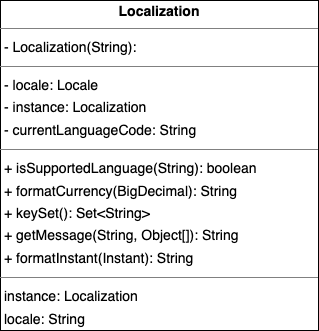
\includegraphics[width=0.5\linewidth]
    {kapitel8_entwurfsmuster/UMLs/localizaition.drawio.png}
\end{figure}

\subsection{Entwurfsmuster: Factory/Builder (Erzeugungsmuster) (4P)}

\textbf{Bezeichnung:} Factory / Builder (statische Factorymethode) \\
\textbf{Einsatz im Projekt:} Klassen wie \texttt{BankAccount}, \texttt{Transaction}, \texttt{User} (z.\,B. \texttt{BankAccount.create()})

\subsection*{Sinnvoller Einsatz}
Objekte wie Bankkonten oder Transaktionen sollen immer im konsistenten Zustand erstellt werden.
Statt viele verschiedene Konstruktoren zu nutzen, wird eine kontrollierte \texttt{create()}-Methode verwendet.
Dadurch wird die Instanziierung vereinfacht und typische Fehler bei der Objekterstellung werden vermieden.


\subsection*{Codebeispiel: Statische Factory-Methode \texttt{create()}}
\lstinputlisting[
    language=Java,style=codeStyle]{kapitel8_entwurfsmuster/code/BankAccount.java}


\subsection*{UML-Diagramm}
\begin{figure}[htbp]
    \centering
    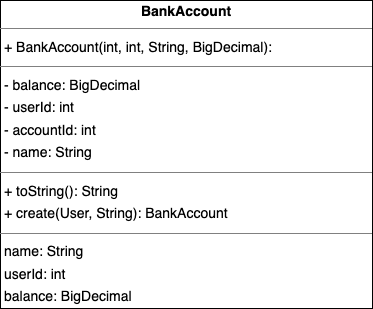
\includegraphics[width=0.6\linewidth]
    {kapitel8_entwurfsmuster/UMLs/BankAccount.drawio.png}
\end{figure}

\subsection*{Begründung}
\begin{itemize}
    \item Einheitliche Instanziierung über statische Fabrikmethoden
    \item Vermeidung fehleranfälliger Konstruktoraufrufe mit falschen Parametern
    \item Möglichkeit zur Vorbelegung von Standardwerten (z.\,B. \texttt{balance = 0})
    \item Erhöhte Lesbarkeit und Wartbarkeit
\end{itemize}